\documentclass[noauthor,nooutcomes,12pt]{ximera}

\graphicspath{  
{./}
{./whoAreYou/}
{./drawingWithTheTurtle/}
{./bisectionMethod/}
{./circles/}
{./anglesAndRightTriangles/}
{./lawOfSines/}
{./lawOfCosines/}
{./plotter/}
{./staircases/}
{./pitch/}
{./qualityControl/}
{./symmetry/}
{./nGonBlock/}
}


%% page layout
\usepackage[cm,headings]{fullpage}
\raggedright
\setlength\headheight{13.6pt}


%% fonts
\usepackage{euler}

\usepackage{FiraMono}
\renewcommand\familydefault{\ttdefault} 
\usepackage[defaultmathsizes]{mathastext}
\usepackage[htt]{hyphenat}

\usepackage[T1]{fontenc}
\usepackage[scaled=1]{FiraSans}

%\usepackage{wedn}
\usepackage{pbsi} %% Answer font


\usepackage{cancel} %% strike through in pitch/pitch.tex


%% \usepackage{ulem} %% 
%% \renewcommand{\ULthickness}{2pt}% changes underline thickness

\tikzset{>=stealth}

\usepackage{adjustbox}

\setcounter{titlenumber}{-1}

%% journal style
\makeatletter
\newcommand\journalstyle{%
  \def\activitystyle{activity-chapter}
  \def\maketitle{%
    \addtocounter{titlenumber}{1}%
                {\flushleft\small\sffamily\bfseries\@pretitle\par\vspace{-1.5em}}%
                {\flushleft\LARGE\sffamily\bfseries\thetitlenumber\hspace{1em}\@title \par }%
                {\vskip .6em\noindent\textit\theabstract\setcounter{question}{0}\setcounter{sectiontitlenumber}{0}}%
                    \par\vspace{2em}
                    \phantomsection\addcontentsline{toc}{section}{\thetitlenumber\hspace{1em}\textbf{\@title}}%
                     }}
\makeatother



%% thm like environments
\let\question\relax
\let\endquestion\relax

\newtheoremstyle{QuestionStyle}{\topsep}{\topsep}%%% space between body and thm
		{}                      %%% Thm body font
		{}                              %%% Indent amount (empty = no indent)
		{\bfseries}            %%% Thm head font
		{)}                              %%% Punctuation after thm head
		{ }                           %%% Space after thm head
		{\thmnumber{#2}\thmnote{ \bfseries(#3)}}%%% Thm head spec
\theoremstyle{QuestionStyle}
\newtheorem{question}{}



\let\freeResponse\relax
\let\endfreeResponse\relax

%% \newtheoremstyle{ResponseStyle}{\topsep}{\topsep}%%% space between body and thm
%% 		{\wedn\bfseries}                      %%% Thm body font
%% 		{}                              %%% Indent amount (empty = no indent)
%% 		{\wedn\bfseries}            %%% Thm head font
%% 		{}                              %%% Punctuation after thm head
%% 		{3ex}                           %%% Space after thm head
%% 		{\underline{\underline{\thmname{#1}}}}%%% Thm head spec
%% \theoremstyle{ResponseStyle}

\usepackage[tikz]{mdframed}
\mdfdefinestyle{ResponseStyle}{leftmargin=1cm,linecolor=black,roundcorner=5pt,
, font=\bsifamily,}%font=\wedn\bfseries\upshape,}


\ifhandout
\NewEnviron{freeResponse}{}
\else
%\newtheorem{freeResponse}{Response:}
\newenvironment{freeResponse}{\begin{mdframed}[style=ResponseStyle]}{\end{mdframed}}
\fi



%% attempting to automate outcomes.

%% \newwrite\outcomefile
%%   \immediate\openout\outcomefile=\jobname.oc
%% \renewcommand{\outcome}[1]{\edef\theoutcomes{\theoutcomes #1~}%
%% \immediate\write\outcomefile{\unexpanded{\outcome}{#1}}}

%% \newcommand{\outcomelist}{\begin{itemize}\theoutcomes\end{itemize}}

%% \NewEnviron{listOutcomes}{\small\sffamily
%% After answering the following questions, students should be able to:
%% \begin{itemize}
%% \BODY
%% \end{itemize}
%% }
\usepackage[tikz]{mdframed}
\mdfdefinestyle{OutcomeStyle}{leftmargin=2cm,rightmargin=2cm,linecolor=black,roundcorner=5pt,
, font=\small\sffamily,}%font=\wedn\bfseries\upshape,}
\newenvironment{listOutcomes}{\begin{mdframed}[style=OutcomeStyle]After answering the following questions, students should be able to:\begin{itemize}}{\end{itemize}\end{mdframed}}



%% my commands

\newcommand{\snap}{{\bfseries\itshape\textsf{Snap!}}}
\newcommand{\flavor}{\link[\snap]{https://snap.berkeley.edu/}}
\newcommand{\mooculus}{\textsf{\textbf{MOOC}\textnormal{\textsf{ULUS}}}}


\usepackage{tkz-euclide}
\tikzstyle geometryDiagrams=[rounded corners=.5pt,ultra thick,color=black]
\colorlet{penColor}{black} % Color of a curve in a plot



\ifhandout\newcommand{\mynewpage}{\newpage}\else\newcommand{\mynewpage}{}\fi

\usepackage{fullpage}
\makeatletter
%% no number for activity
\newcommand\logostyle{%
  \def\activitystyle{activity-chapter}
  \def\maketitle{%
                {\flushleft\small\sffamily\bfseries\@pretitle\par\vspace{-1.5em}}%
                {\flushleft\LARGE\sffamily\bfseries\@title \par }%
                {\vskip .6em\noindent\textit\theabstract\setcounter{problem}{0}\setcounter{sectiontitlenumber}{0}}%
                    \par\vspace{2em}
                    \phantomsection\addcontentsline{toc}{section}{\textbf{\@title}}%
                     \setcounter{titlenumber}{0}}}
\makeatother
\newcommand{\nameblankgen}{\noindent\textbf{Name(s) (please print):}\ \hrulefill \\

\hrulefill}
\logostyle



\title{Arguments and inputs}
\author{Bart Snapp}

\begin{document}
\begin{abstract}
  We make functions with inputs.
\end{abstract}
\maketitle

\nameblankgen

\begin{multicols*}{2}

  Let me remind you how to draw a regular $n$-gon \lc{repeat :n [ fd
      :s rt 360/:n ]}, where \lc{:n} and \lc{:s} are variables that
  YOU are supposed to fill in. Variables that friends are supposed to
  provide are called \dfn{arguments}.  We can make \LOGO\ functions
  with arguments easily. As a gesture of friendship, let me present you with \lc{reg.n.gon :n :s}
\begin{logo}
to reg.n.gon :n :s
  repeat :n [ fd :s rt 360/:n ]
end
\end{logo}
With that code, we can use \lc{reg.n.gon 3 200} to make an equilateral
triangle. In fact we can do something \emph{really cool} we can
write new functions \textit{in terms of this function.} For example:
\begin{logo}
to eq.tri :s reg.n.gon 3 :s end
to square :s reg.n.gon 4 :s end
to circle reg.n.gon 360 1.74538 end
\end{logo}

\section{Loading programs}

Once you have a file with all of these functions, we can load these
functions into \emph{any} \LOGO\ activity with the \lc{include}
command. Here's how it works, every Turtle Academy program has a
unique URL that looks something like:
\[
\texttt{https://turtleacademy.com/programs/12345}
\]
to load this program in another program, you simply do something like:
\begin{logo}
include 12345
square 100  
\end{logo}
and the program associated to ``12345'' will be loaded, and you can
then use the functions within.


\section{Many variables}

We could also make a (very basic) \lc{cannon} command. Check this out:

\begin{logo}
to cannon :h :f :r :t
seth 90 rt -:h
setwidth 10
  repeat :t [
    setcolor 5*repcount/:t
    fd :f rt :r ]
end
\end{logo}
Note, this function has \textsc{four} arguments. We can see the flight
of a ``cannon ball'' with this function as \lc{cannon 60 3 1 120} produces:
\begin{logoout}
  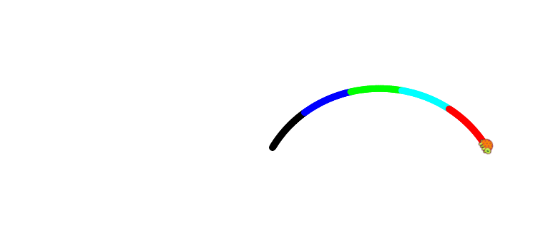
\includegraphics[width=.4\textwidth]{cannon.png}
\end{logoout}
You may wonder, where did the cannon ball land? You can use \lc{print
  xcor} and \lc{print ycor} to figure this out.


\section{Commands to know}
\begin{tabular}{lll}
  \lc{CMD}   & Description      & Example           \\ \hlinewd{1pt}
  \lc{include \#} & input a library & \lc{include 12345} \\
  \lc{xcor} & horizontal position & \lc{print xcor} \\
  \lc{ycor}     & vertical position & \lc{print ycor}\\
  \lc{heading} & current heading  & \lc{print heading}
\end{tabular}
\end{multicols*}

\newpage

\begin{problem}
  Make a new program and call it \lc{Library}.  Add our functions
  \lc{reg.n.gon}, \lc{eq.tri}, \lc{square}, \lc{circle} to your
  library. Add \emph{two} new routines that make basic shapes to your program
  \lc{Library}. Show-off your work with your code and a picture. 
\end{problem}

\mynewpage

\begin{problem}
  Enhance your program \lc{circle} so that it has its radius as an input,
  and will draw a circle of radius \lc{:r}.  Use \lc{print},
  \lc{xcor}, and \lc{ycor} to show that your code works. Show-off your
  work with your code and a picture.
\end{problem}

\mynewpage


\begin{problem}
  Make an \lc{rainbow :w} command that will make a rainbow of a given
  width centered around a point.
\end{problem}

\mynewpage

\begin{problem}
  Make an \lc{arrow :h :l :p} command that will take a heading
  \lc{:h}, a length for the arrow shaft \lc{:l}, and \lc{:p} will give
  the size of the pointy-end.  Show-off your work with your code and a
  picture.
\end{problem}

\mynewpage

\begin{problem}
  Imagine a ``cannon'' is sitting at $(0,0)$ and that there is a
  ``target'' at $(150,0)$. Use \lc{print xcor} to hit the target with
  \lc{cannon 60 :f 1 120} by modifying \lc{:f}.

  \emph{Keep track of how many attempts it takes you to hit the target
    to within one decimal place.}

  Present your attempts as data, with \emph{Attempt number}, \lc{:f},
  \lc{xcor} as headings.
\end{problem}








\end{document}
